\documentclass[journal]{IEEEtran}
\usepackage{amsmath,amssymb,amsfonts}
\usepackage{graphicx}
\usepackage{booktabs}
\usepackage{multirow}
\usepackage[ruled,vlined,linesnumbered]{algorithm2e}
\usepackage{tikz}
\usetikzlibrary{arrows.meta,positioning,shapes.geometric,fit,backgrounds}
\usepackage[colorlinks=true,linkcolor=blue,citecolor=blue,urlcolor=blue]{hyperref}
\usepackage{xcolor}
\hypersetup{
  pdftitle={Regime-Dependent Rebalancing for UAV Object Detection: An Exposure-Aware Data-Centric Study},
  pdfauthor={Nu Wen, Ying Zhou, Chongchong Yao, and Yebin Chen},
  pdfsubject={UAV object detection},
  pdfkeywords={UAV object detection, long-tailed recognition, small-object detection, data-centric AI, VisDrone, UAVDT}
}

\newcommand{\map}{\ensuremath{\mathrm{mAP}}}
\newcommand{\ap}{\ensuremath{\mathrm{AP}}}
\newcommand{\apf}{\ensuremath{\mathrm{AP}_{50}}}
\newcommand{\aps}{\ensuremath{\mathrm{AP}_{s}}}
\newcommand{\remdet}{RemDet-X}
\newcommand{\visdrone}{VisDrone2019-DET}
\newcommand{\uavdt}{UAVDT}
\newcommand{\dahpL}{DAHP-L}
\newcommand{\dahpM}{DAHP-M}

\begin{document}

\title{Regime-Dependent Rebalancing for UAV Object Detection: An Exposure-Aware Data-Centric Study}

\author{Nu~Wen, Ying~Zhou, Chongchong~Yao, and Yebin~Chen%
\thanks{Nu Wen is with the Internet of Things Research Institute, Shenzhen Polytechnic University, Shenzhen 518055, China (e-mail: wennu1989@gmail.com).}%
\thanks{Ying Zhou is with the Internet of Things Research Institute, Shenzhen Polytechnic University, Shenzhen 518055, China, and also with the School of Architecture and Urban Planning, Shenzhen University, Shenzhen 518060, China.}%
\thanks{Chongchong Yao is with the Internet of Things Research Institute, Shenzhen Polytechnic University, Shenzhen 518055, China, and also with the School of Geography Science and Geomatics Engineering, Suzhou University of Science and Technology, Suzhou 215009, China.}%
\thanks{Yebin Chen is with the School of Architecture and Urban Planning, Shenzhen University, Shenzhen 518060, China (corresponding author, e-mail: chenyebin@szu.edu.cn).}%
\thanks{Code, configurations, per-class results, and failure audits are available from the public repository stated in the Data and Code Availability section.}}

\maketitle

\begin{abstract}
UAV imagery presents three coupled distributional pathologies: 85.3\% of instances are smaller than $32{\times}32$ pixels at a 640-px reference, the head-to-tail class ratio is approximately $45{:}1$, and 23 class pairs exceed a structural-confusion threshold. We first audit a three-component feature-module family---cross-scale attention, class-conditioned attention, and frequency-balanced enhancement---in seven matched 100-epoch variants; they increase validation DFL and change $\map_{50\text{-}95}$ by only $-0.7$ to $+0.1$~\ap, providing no reliable improvement. We then introduce DAHP, a label-only profiling mechanism followed by a bounded policy search, which maps long-tail, scale, and structural-confusion statistics to candidate effective-pixel configurations, union oversampling, and optional fusion. The central empirical contribution is an exposure-aware regime-dependent rebalancing principle: volume dominates under-fitted regimes, random duplication is nearly neutral when volume is saturated, both channels contribute in an intermediate window, and apparent high-resolution gains can largely reflect additional exposure. At 1920\,px, exposure matching reduces an apparent $+3.83$-\ap{} gain to $+0.42$~md100 \ap. On VisDrone val, DAHP-L reaches $38.16$~md100 \ap{} and $40.06$~native \ap{} under the disclosed 1600-px/P2 policy. The same-input DAHP-M control exceeds modern YOLO baselines but not D-FINE-M or RT-DETRv2-L, and a matched RT-DETR probe is negative; thus, the policy claim is bounded to the studied YOLO family. The recipe transfers to UAVDT ($+0.69$~\ap; tail $+1.69$). On an exclusive desktop RTX~3090, a 300-image stage-wise protocol measures $38.0$~ms end-to-end ($26.3$~FPS) with separate preprocessing, inference, post-processing, and memory accounting.
\end{abstract}

\begin{IEEEkeywords}
UAV object detection, long-tailed recognition, small-object detection, data-centric AI, training-regime analysis, VisDrone, UAVDT.
\end{IEEEkeywords}

\section{Introduction}
\IEEEPARstart{A}{erial} imagery acquired from low-altitude UAV platforms poses a detection problem that is structurally distinct from ground-level benchmarks. An audit of the \visdrone{} training labels (6{,}471 images, 343{,}204 instances; the 548-image validation split is reserved for evaluation) reveals three coupled pathologies:

\subsection{Three Coupled Pathologies}

\subsubsection{Scale imbalance} At the standard 640-px reference, 85.3\% of instances are smaller than $32{\times}32$ pixels and 58.0\% smaller than $16{\times}16$ (58.0\%/23.4\% at the 1280-px training reference); object scales span three orders of magnitude, so any single receptive-field configuration is mismatched to most of the data.

\subsubsection{Long-tailedness} The head class (\emph{car}) outnumbers the rarest non-empty class (\emph{awning-tricycle}) by $44.6{:}1$; the threshold-defined tail set contains \emph{tricycle}, \emph{awning-tricycle}, and \emph{bus}, whose diversity cannot be learned under uniform sampling.

\subsubsection{Inter-class confusion} Twenty-three category pairs exceed $0.85$ on an annotation-level structural-similarity proxy $\kappa$ (Sec.~\ref{sec:method}); the head-anchored confusion axis concentrates on \emph{car--van--truck}.

These pathologies are not independent: tail classes are also the smallest on average and the most confusable (Fig.~\ref{fig:profile}). Interventions that address one factor in isolation risk being confounded---or counteracted---by the other two.

\begin{figure*}[!t]
\centering
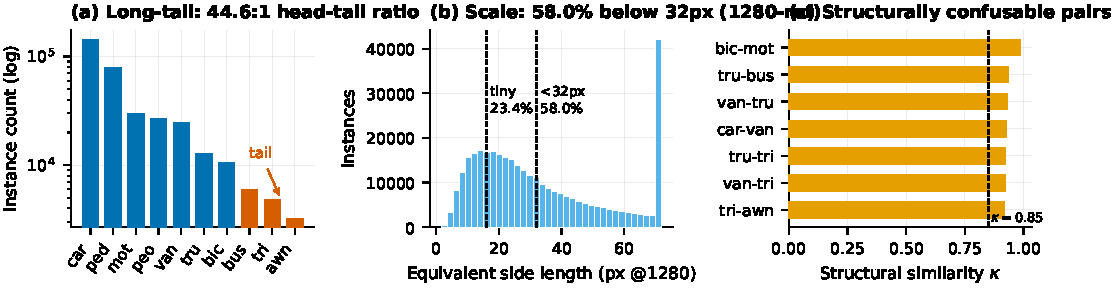
\includegraphics[width=\textwidth]{figures/fig1_factor_stats.pdf}
\caption{Label-only pathology profile of the \visdrone{} training set. (a) Instance frequency spans a 44.6:1 head-to-tail ratio. (b) At the 1280-px reference, 58.0\% of instances are smaller than $32{\times}32$ pixels and 23.4\% smaller than $16{\times}16$; at 640\,px the corresponding small-object fraction is 85.3\%. (c) The annotation-level structural-confusion proxy $\kappa$ identifies confusable category pairs; the dashed line marks the reported graph threshold $\kappa=0.85$.}
\label{fig:profile}
\end{figure*}

\subsection{The Architectural Turn and Its Missing Evidence}
The dominant community response has been architectural: density-guided cropping \cite{clusdet,dmnet,ufpmp}, small-object heads \cite{tph,sahi}, and specialized detectors \cite{remdet,uavdetr}. This trend compounds design elements already embedded in strong dense detectors, including focal/quality-aware assignment, multi-level anchor-free prediction, distributional box regression, and deformable sampling \cite{focal,fcos,gfl,deform}. Each reports gains, yet three gaps persist. First, comparisons frequently co-vary input resolution, schedule, and capacity---precisely the variables that dominate UAV accuracy. Second, negative results are rarely reported, preventing the community from distinguishing ``module~A helps'' from ``module~A was tested once, on a weak baseline.'' Third, the interaction between data-level rebalancing and the training regime---\emph{when} rebalancing helps---has not been characterized.

\subsection{Contributions}
\begin{enumerate}
\item \textbf{A controlled negative-result study} (a three-component feature-module family in seven matched variants, $20+$ audited trainings; Table~\ref{tab:negative}): feature-level interventions systematically elevate validation DFL and fail to improve $\map_{50\text{-}95}$ on strong baselines, including head-level decoupling attempts (Sec.~\ref{sec:negative}).
\item \textbf{The regime-dependent rebalancing principle}: using an epoch-matched resolution ladder and factor-isolated sampling controls, we formalize regimes in which rebalancing behaves as volume-driven tail rescue, volume-saturated reallocation with a bounded targeted residual, positive-sum augmentation, or an exposure-limited apparent gain, yielding an operational decision rule (Sec.~\ref{sec:principle}).
\item \textbf{A non-invasive data profiling and bounded policy-search mechanism (DAHP)}: a label-only profiler emits a resolution ladder, tail and confusion-axis oversampling, and optional fusion candidates; bounded base/random probes, memory feasibility, and exposure evidence then select the final policy. The rebalancing policy leaves stock losses and inference unchanged. The identical profiler transfers zero-shot to \uavdt{}---a profiler transfer, with the final policy still subject to the disclosed bounded search---where the observed factor attribution is consistent with its label profile (Sec.~\ref{sec:method}, \ref{sec:uavdt}).
\item \textbf{Protocol-faithful comparator evidence} across more than 25 detector configurations, including reproduced YOLO11/YOLO12/YOLO26, D-FINE, RT-DETRv2, and UAV-specific detectors. Exposure-matched and volume-matched controls separate architecture, data volume, and targeted rebalancing; the P2 ladder is re-evaluated under one native protocol, the 1920-\ap{} gain is decomposed into exposure and residual components, and a matched RT-DETR probe is explicitly reported as a negative family-boundary result (Sec.~\ref{sec:main}--\ref{sec:attribution}).
\end{enumerate}

\section{Related Work}
\subsection{UAV Object Detection}
\subsubsection{Cropping and packing pipelines}
ClusDet \cite{clusdet} clusters dense regions and discards background, trading coverage for effective pixels; DMNet \cite{dmnet} learns a density map to guide cropping; UFPMP-Det \cite{ufpmp} unifies foreground packing with multi-proxy reassembly; CZDet \cite{czdet} cascades density-guided zoom-in over high-resolution aerial images; AMRNet \cite{amrnet} augments aerial chips with scale-adaptive chip generation, mosaic augmentation, and mask resampling. These pipelines demonstrate the value of pixels per object, but they complicate attribution: any reported gain bundles the cropping policy, the effective resolution gain it induces, and the detector itself. Our controlled ladders (Table~\ref{tab:ladder}) measure the resolution effect alone, and our negative result on pure tiled inference (Sec.~\ref{sec:negative}) shows that cropping applied \emph{only at inference} is harmful on full-image-trained models---consistent with a train--test scale-distribution mismatch rather than an intrinsic property of cropping.
\subsubsection{Detector-side designs}
TPH-YOLOv5 \cite{tph} adds transformer prediction heads for small objects; \remdet{} \cite{remdet} rethinks efficient UAV detector design via ChannelC2f, GatedFFN, and the CED downsampling module; UAV-DETR \cite{uavdetr}, DOL-DETR \cite{doldetr}, LGI-DETR \cite{lgidetr}, and AQF-Net \cite{aqfnet} introduce detector families or query/feature designs tailored to UAV imagery; UAVDet \cite{uavdetmamba} couples CNN and Mamba blocks in a tiny-focused feature pyramid, and CASA-Net \cite{casanet} adapts context modeling, label assignment, and aerial-specific augmentation for UAV small objects. These are architecture-first contributions. What they leave open is threefold: (i) whether their gains persist when a strong baseline is given the same resolution and budget (our compute-matched \remdet{} retrain probes exactly this); (ii) whether data-level policies improve a strong baseline once resolution and capacity are disclosed rather than hidden (our full policy does, with $58\%$ of \remdet{}'s parameters); and (iii) \emph{when} any rebalancing helps---the regime question this paper answers.
\subsubsection{Slicing-aided fine-tuning}
SAHI \cite{sahi} fine-tunes on tiles to align train--test scale distributions. Our SAFT experiments confirm the alignment is necessary (pure sliced inference is $-2.3$ to $-2.6$~\ap), but also show that a naive mixture underperforms pure test-time augmentation ($37.76$ vs.\ $37.96$), motivating our choice of full-image training at matched effective pixels instead.

\subsection{Long-Tailed Detection}
Loss-space methods---class-balanced reweighting \cite{cbloss}, margin-aware losses \cite{ldam}, EQLv2 \cite{eqlv2}, Seesaw \cite{seesaw}, balanced group softmax \cite{bge}, and distribution-balanced losses \cite{dbloss}---modify gradients; data-space methods such as repeat-factor sampling \cite{rfs} and aerial chip augmentation \cite{amrnet} replicate or synthesize tail examples. Closest to our setting, AD-Det \cite{addet} jointly addresses focused small objects and balanced tail classes through a coarse-to-fine architecture and dynamic class-balanced copy-paste, while E-IRFS \cite{eirfs} designs exponentially weighted instance-aware repeat factors for long-tailed UAV training. These works engineer stronger interventions; we instead hold the detector fixed and ask \emph{when} a rebalancing intervention helps at all, separating volume, targeted reallocation, and exposure effects under matched budgets. Our negative results extend to loss-space interventions on strong baselines, and the regime principle (Sec.~\ref{sec:principle}) explains why: once the volume channel is saturated, indiscriminate reweighting is approximately zero-sum. Unlike prior work, we characterize \emph{when} rebalancing is positive-sum, using the training regime as the moderator.

\subsection{Scale and Resolution}
Resolution is the largest single lever in UAV detection (our historical ladders: $+8.8$~\ap{} from $640{\to}1280$). QueryDet \cite{querydet} and CEASC \cite{ceasc} accelerate high-resolution inference through sparse-query and context-enhanced adaptive sparse convolution, respectively; Gold-YOLO \cite{goldyolo} and RT-DETR \cite{rtdetr} advance general-purpose accuracy. We contribute an epoch-matched, \emph{non-monotonic} resolution curve peaking at $1600$\,px with a $2.8$-\ap{} drop at $1920$\,px under fixed compute---to our knowledge not previously documented under controlled epochs.

\subsection{Reporting Practice}
Dual-protocol evaluation (\emph{maxDets} $100/300$) is motivated by \visdrone{} density (64.8\% of images exceed 50 objects; up to 317 instances) \cite{visdrone}. Weighted-box fusion \cite{wbf} aggregates model families. We report per-class \ap{} for every configuration and disclose all failures.

\section{Method}
\label{sec:method}
\subsection{Problem Formulation and Three-Factor Profiling}
Let $\mathcal{D}=\{(x_i,Y_i)\}_{i=1}^{N}$ denote the training set with class set $\mathcal{C}$, $|\mathcal{C}|=K$. DAHP computes, from labels alone:

\emph{(i) Frequency factor.} The class distribution and tail set are
\begin{equation}
f(c)=\frac{N_c}{\sum_{c'} N_{c'}},\qquad
\mathcal{T}=\{c\in\mathcal{C}: N_c < 0.3\,\overline{N}\},
\label{eq:tail}
\end{equation}
where $N_c=\sum_i\mathbf{1}[c\in Y_i]$, $\overline{N}$ is the mean over non-empty classes, and the imbalance ratio is $\rho=\max_c N_c/\min_{c\in\mathcal{T}}N_c$.

\emph{(ii) Scale spectrum.} With $\sigma(c)$ the equivalent side length of class-$c$ instances at a reference resolution $r$,
\begin{equation}
s_{\mathrm{small}}(c)=\Pr\big[\sigma(c)<32\big],\quad
s_{\mathrm{tiny}}(c)=\Pr\big[\sigma(c)<16\big],
\label{eq:scale}
\end{equation}
and the frequency-weighted scale masses are $m_{\mathrm{small}}=\sum_c f(c)s_{\mathrm{small}}(c)$ and $m_{\mathrm{tiny}}=\sum_c f(c)s_{\mathrm{tiny}}(c)$. A P2 (high-resolution) head is recommended when $m_{\mathrm{small}}>0.3$.
Because profiling does not decode images, $\sigma$ is computed in a square
reference space from normalized label extents; it is a policy statistic for
ranking configurations, not a sensor-calibrated physical length.

\emph{(iii) Confusion graph.} A pairwise annotation-level \emph{structural confusion proxy}
\begin{equation}
\kappa(a,b)=\lambda\,J_{\mathrm{ar}}(a,b)+(1-\lambda)\,J_{s}(a,b),\qquad \lambda=0.6,
\label{eq:conf}
\end{equation}
where $J_{\mathrm{ar}}$ and $J_{s}$ are histogram intersections of the aspect-ratio and instance-scale ($s{=}w_r h_r$) distributions at the reference resolution. Edges with $\kappa>0.85$ form the confusion graph; the oversampling axis is its head-anchored neighborhood $\mathcal{A}=\{c\notin\mathcal{H}\cup\mathcal{T}:\kappa(c,h)>\tau_A\}$ for head set $\mathcal{H}=\{c:N_c>\overline{N}\}$ and margin $\tau_A{=}0.86$ (which excludes the borderline semantic near-duplicate \emph{people--pedestrian} pair at $\kappa{=}0.854$). Co-occurrence Jaccard is additionally reported as an auxiliary statistic but does not enter $\kappa$.

\emph{(iv) Density profile.} Instances per image justify the \emph{maxDets}$=300$ evaluation protocol for dense scenes.

On \visdrone{} the profiler yields $(\rho{=}45{:}1,\ 58.0\%\ \text{small at the 1280-px reference},\ 23\ \text{pairs}>0.85,\ \mathcal{A}=\{\text{van},\text{truck}\})$; on \uavdt{}---without any change---$(\rho{=}30.7{:}1,\ 74.8\%\ \text{small at 640-px},\ \text{car--van}\ 0.935,\ \mathcal{A}=\{\text{van}\})$.

Because $\lambda$ and $\tau=0.85$ are decision boundaries rather than fitted parameters, we also release a label-only sensitivity audit (Appendix Table~\ref{tab:thresholds}). The VisDrone tail set is unchanged for all $12$ combinations of $\lambda\in\{0.4,\ldots,0.7\}$ and $\tau\in\{0.80,0.85,0.90\}$, and \emph{van} remains on the confusion axis in every case. The reported operating point is locally stable for $\lambda\in\{0.6,0.7\}$ at $\tau=0.85$ ($\mathcal{A}=\{\text{van},\text{truck}\}$); a conservative $\tau=0.90$ removes \emph{truck}, while a permissive $\tau=0.80$ admits additional mid-frequency classes. On \uavdt{}, the selected policy $\{\text{truck},\text{bus},\text{van}\}$ is identical over the entire grid. The head-anchored eligibility margin is likewise not independently fitted: in the released audit $\tau_A$ is tied to the graph threshold by a conservative $+0.01$ margin, so the tested pairs are $(\tau,\tau_A)\in\{(0.80,0.81),(0.85,0.86),(0.90,0.91)\}$. This audit establishes decision stability and discloses its boundaries; it is not an AP sweep, because each alternative sampling set was not trained.

\subsection{The Regime-Dependent Rebalancing Principle}
\label{sec:principle}
Define the epoch-wise aggregate gain $g(e)=\map(e)-\map(e{-}1)$ and its windowed mean $\bar{g}(E)=\frac{1}{W}\sum_{e=E-W+1}^{E}g(e)$. A configuration is
\begin{equation}
\textit{under-fitted}\ \Leftrightarrow\ \bar{g}(E)>\tau_g;\qquad
\textit{saturated}\ \Leftrightarrow\ |\bar{g}(E)|\le\tau_g,
\label{eq:regime}
\end{equation}
with $\tau_g$ a small threshold (0.1~pt, $W{=}10$); otherwise it is \emph{intermediate}. Let $h$ denote \emph{data-exposure headroom}, estimated by the gain of a volume-matched random-duplication arm, and let $\Delta_{\mathrm{vol}}$ and $\Delta_{\mathrm{dir}}$ denote the aggregate-\ap{} contributions of pure volume and targeted class reallocation. Define $\Delta_{\mathrm{se}}$ and $\Delta_{\mathrm{m}}$ as the same-epoch and exposure-matched union gains.

The labels in Eq.~\eqref{eq:regime} are descriptive summaries of completed controlled runs, not a claim that a single training curve identifies the regime online. The operative decision variable is $h$: in the completed controls, the base/random two-arm comparison estimates whether additional exposure was still convertible into accuracy before the targeted policy is interpreted (Sec.~\ref{sec:earlysignal}). Our controlled observations support:
\begin{align}
\text{P1 (under-fit)} &\Rightarrow \tfrac{\Delta_{\mathrm{vol}}}{\Delta_{\mathrm{vol}}+\Delta_{\mathrm{dir}}}\approx0.96,\ \Delta\ap_{\mathrm{tail}}>0;\\
\text{P2 (volume-sat.)} &\Rightarrow \Delta_{\mathrm{vol}}\approx0,\ 0\le\Delta_{\mathrm{dir}}\lesssim0.5,\\
&\qquad \exists(c)\!:\!\Delta\ap_c<0;\\
\text{P3 (intermediate)} &\Rightarrow 0<\Delta\ap_{\mathrm{agg}}\le 1.0,\ \Delta_{\mathrm{vol}},\Delta_{\mathrm{dir}}>0;\\
\text{P4 (exposure-lim.)} &\Rightarrow \Delta_{\mathrm{se}}\gg\Delta_{\mathrm{m}},\ \Delta\ap_s^{(\mathrm{m})}>0.
\end{align}
The principle yields the operational rule: \emph{profile whether a plateau is caused by capacity, learnability, or exhausted exposure; rebalance when exposure headroom or an intermediate positive-sum window exists, and do not interpret a same-epoch high-resolution gain as targeted rebalancing until exposure is matched.}

\subsection{Policy Mapping and Bounded Configuration Search}
\subsubsection{Computational cost}
DAHP is deliberately label-only: profiling a 6{,}471-image training set requires $O(N)$ label parsing ($<1$\,s on CPU) and $O(K^2)$ pairwise statistics; the policy mapping itself is constant-time. No images are decoded, no gradients are computed, and no detector forward pass is needed. This contrasts with profiling approaches that require model inference (e.g., error-driven confusion mining), and it makes the engine directly portable---the same code produced both the VisDrone and UAVDT policies without dataset-specific edits.

\subsubsection{Why a data-space probe rather than loss reweighting}
Long-tailed detection conventionally intervenes in the loss through reweighting or logit adjustment. The regime controls identify when such an intervention can be insufficient: once the volume channel is saturated, an untargeted loss change reallocates a fixed optimization budget but does not create additional useful exposure. Data-space duplication, by contrast, explicitly changes the exposure available to the data loader and augmentation pipeline. Its random-volume component isolates that exposure effect, while the union policy in Eq.~\eqref{eq:weight} adds class-targeted reallocation. This decomposition is why the base/random control is part of the policy rather than an afterthought.

\subsubsection{Configuration nomenclature}
Throughout the paper we use a systematic configuration shorthand. \textbf{R} denotes the effective-pixel policy (resolution/backbone selection from the regime curve); \textbf{T} the tail-class oversampling of $\mathcal{T}$; \textbf{C} the confusion-axis oversampling of $\mathcal{A}$; and \textbf{B} the backbone scale-up (v8m$\to$v8l). The shorthand composes: e.g., R$+$T$\cup$C applies resolution plus union oversampling. Two named models recur: \dahpM{} (YOLOv8m-P2 with R$+$T$\cup$C; input is stated per table row---640 for the same-input control and 1600 for the component ablation) and \dahpL{} (YOLOv8l-P2@1600, R$+$T$\cup$C)---the latter is the primary full-capacity single model---plus \dahpL{}-E7, the seven-model weighted-box-fusion ensemble. Architecture-decomposition controls are written $V_L$ (vanilla v8l, no P2 head) and $V_L{+}P_2$.

Resolution selection requires this distinction: \emph{profiling} is label-only,
but the final input size is a bounded policy search subject to memory and the
regime probe. The profiler returns the candidate ladder
$\{960,1280,1600,1920\}$ and a tiny-object-mass prior (implemented thresholds:
$m_{\mathrm{tiny}}>0.55,0.35,0.15$ map to $1920,1600,1280$\,px, respectively;
otherwise $960$\,px); short base/random probes may then reject an
exposure-poor or unlearnable candidate. For \visdrone{}, the 640-reference
profile has $m_{\mathrm{tiny}}=0.580$, so the label-only prior initially points
to 1920\,px; bounded probes and the memory-constrained non-monotonic ladder
retain 1600\,px. \uavdt{} remains within its 640-px reference budget. We do
not claim that the best resolution is computable from labels alone.

The oversampling weight of image $x_i$ under the union policy is
\begin{equation}
w_i = 1 + \mathbf{1}\big[(Y_i\cap(\mathcal{T}\cup\mathcal{A}))\neq\varnothing\big],
\label{eq:weight}
\end{equation}
i.e., any image containing a tail or confusion-axis class is duplicated. The optional fusion of $M$ models merges boxes $\{b_m\}$ with scores $\{s_m\}$ by
\begin{equation}
\tilde{b}=\frac{\sum_m \tilde{s}_m b_m}{\sum_m \tilde{s}_m},\qquad
\tilde{s}=\frac{1}{|M_c|}\sum_{m\in M_c}s_m,
\label{eq:wbf}
\end{equation}
over IoU-clustered groups $M_c$. The complete procedure is summarized in Algorithm~\ref{alg:dahp}.

\begin{algorithm}[!t]
\caption{DAHP: profile, map, and train. Oversampling is policy-non-invasive; P2/resolution selection is an explicitly disclosed detector configuration.}
\label{alg:dahp}
\KwIn{Labels $\{(Y_i)\}$; detector $\Phi$; budget $E$, batch $B$}
\KwOut{Trained model(s) $\{\Phi^\ast\}$}
\BlankLine
\tcc{--- Stage 1: label-only profiling ---}
compute $N_c$, $\mathcal{T}$, $\rho$ by Eq.~\eqref{eq:tail}\;
compute $s_{\mathrm{small}}, s_{\mathrm{tiny}}$ by Eq.~\eqref{eq:scale}\;
build confusion axis $\mathcal{A}$ by Eq.~\eqref{eq:conf}\;
\tcc{--- Stage 2: regime-aware policy ---}
\eIf{$\sum_c f(c)\,s_{\mathrm{small}}(c)>0.3$}{
  select high-resolution head (P2)\;
}{
  standard head\;
}
rank the ladder $\{960,1280,1600,1920\}$ by tiny-object mass and memory feasibility;\ run bounded base/random probes when budget permits and pick $r^\ast$ in the intermediate regime (Eq.~\eqref{eq:regime})\;
compute image weights $w_i$ by Eq.~\eqref{eq:weight}\;
\tcc{--- Stage 3: non-invasive training ---}
train $\Phi$ on the weighted (duplicated) dataset with \emph{stock} losses and augmentations for $E$ epochs\;
\If{fusion desired}{
  train the family $\{\Phi_m\}_{m=1}^{M}$ and merge by Eq.~\eqref{eq:wbf}\;
}
\Return{$\{\Phi^\ast\}$}\;
\end{algorithm}

\section{Experiments}
\label{sec:experiments}
\subsection{Setup and Protocols}
\visdrone{} \cite{visdrone} (6{,}471 train / 548 val, 10 classes); \uavdt{} \cite{uavdt} (2{,}443 / 641, 4 vehicle classes). DAHP/YOLO-controlled trainings use one RTX~3090, identical augmentation, and disclosed budgets/best epochs; external detector families retain their native recipes as disclosed in Table~\ref{tab:main}. Evaluation uses the standalone COCO-style protocol \cite{coco} (conf $0.001$, NMS-IoU $0.7$) under \emph{dual maxDets}---$100$ for external comparability, $300$ reflecting \visdrone{} density.

\subsubsection{Fairness policy}
We separate what \emph{must} match from what \emph{should stay native}. Matching are: the training set, the validation split, the evaluation protocol (dual \emph{maxDets}), the epoch budget (100 for main rows; disclosed per row otherwise), and the hardware class (single 3090). Native are: each detector's loss functions, optimizer, LR schedule, and augmentation pipeline---these are constitutive parts of a method, and forcing them to be identical would disable exactly the mechanisms under comparison; the same policy is adopted by \remdet{} \cite{remdet} and standard detection benchmarks. Resolution and batch are disclosed per row and additionally \emph{controlled} through three devices: (i) same-detector resolution ladders (Table~\ref{tab:ladder}); (ii) a compute-matched strong-comparator retrain at our resolution (\remdet{}@1600, batch 1 being the physical limit of a 24-GB GPU at that size); and (iii) our full method evaluated \emph{at the baseline resolution} (DAHP-M@640), so that no claimed advantage rests on resolution alone. External numbers transcribed from the literature are marked ``Lit.'' with their split; their exact recipes differ and are cited rather than re-implemented.

\begin{figure*}[!t]
\centering
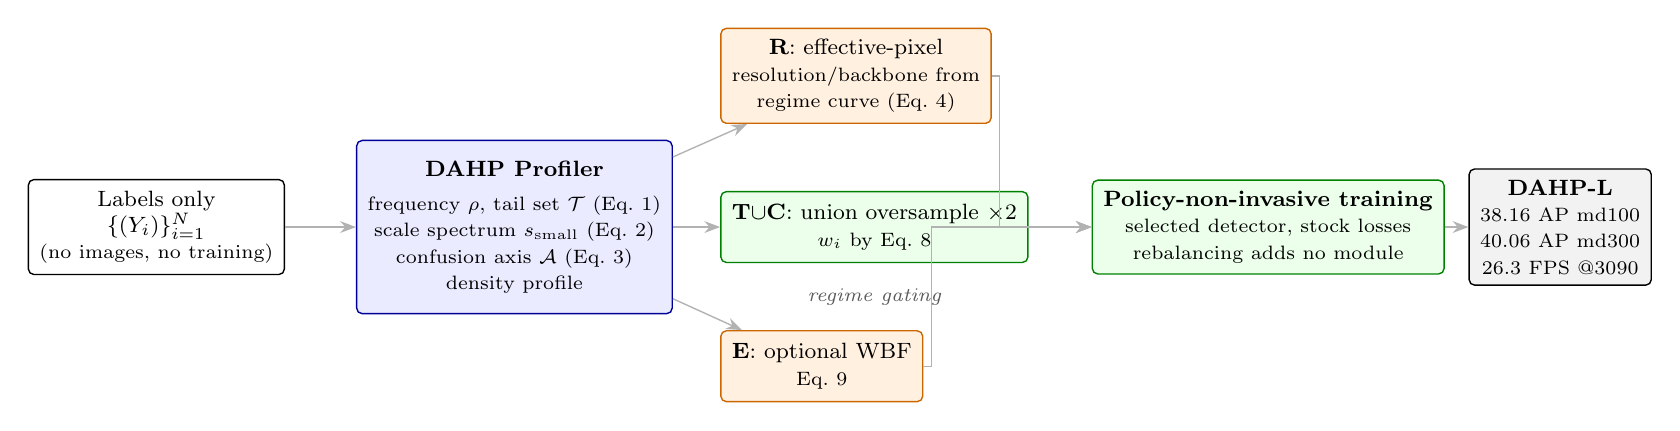
\begin{tikzpicture}[
  font=\footnotesize,
  box/.style={draw, rounded corners=2pt, align=center, minimum height=9mm, inner sep=4pt, line width=0.5pt},
  prof/.style={box, fill=blue!8, draw=blue!60!black},
  pol/.style={box, fill=orange!12, draw=orange!80!black},
  tr/.style={box, fill=green!8, draw=green!50!black},
  ev/.style={box, fill=gray!10},
  arr/.style={-{Stealth[length=2mm]}, line width=0.5pt, draw=gray!60},
  lab/.style={font=\scriptsize\itshape, text=gray!70!black}
]
\node[box] (data) {Labels only\\$\{(Y_i)\}_{i=1}^N$\\{\scriptsize (no images, no training)}};
\node[prof, right=9mm of data, minimum height=22mm] (dahp) {\textbf{DAHP Profiler}\\[1mm]
  {\scriptsize frequency $\rho$, tail set $\mathcal{T}$ (Eq.~1)}\\
  {\scriptsize scale spectrum $s_{\mathrm{small}}$ (Eq.~2)}\\
  {\scriptsize confusion axis $\mathcal{A}$ (Eq.~3)}\\
  {\scriptsize density profile}};
\node[pol, above right=2mm and 6mm of dahp] (res) {\textbf{R}: effective-pixel\\{\scriptsize resolution/backbone from}\\{\scriptsize regime curve (Eq.~4)}};
\node[tr, right=6mm of dahp] (uni) {\textbf{T$\cup$C}: union oversample $\times2$\\{\scriptsize $w_i$ by Eq.~8}};
\node[pol, below right=2mm and 6mm of dahp] (ens) {\textbf{E}: optional WBF\\{\scriptsize Eq.~9}};
\node[tr, right=8mm of uni] (train) {\textbf{Policy-non-invasive training}\\{\scriptsize selected detector, stock losses}\\{\scriptsize rebalancing adds no module}};
\node[ev, right=3mm of train] (eval) {\textbf{\dahpL{}}\\{\scriptsize 38.16 \ap{} md100}\\{\scriptsize 40.06 \ap{} md300}\\{\scriptsize 26.3 FPS @3090}};
\draw[arr] (data) -- (dahp);
\draw[arr] (dahp) -- (res);
\draw[arr] (dahp) -- (uni);
\draw[arr] (dahp) -- (ens);
\draw[arr] (res.east) -- ++(1mm,0) |- (train);
\draw[arr] (uni) -- (train);
\draw[arr] (ens.east) -- ++(1mm,0) |- (train);
\draw[arr] (train) -- (eval);
\node[lab, below=2mm of uni] {regime gating};
\end{tikzpicture}
\caption{The DAHP policy pipeline. A label-only profiler quantifies the three pathologies and maps them, through the regime-dependent rebalancing principle, to training-time sampling and configuration policies; the rebalancing operation itself adds no inference-time module.}
\label{fig:framework}
\end{figure*}

\subsection{Comparison With Reproduced and Reported Detectors}
\label{sec:main}
\begin{table*}[!t]
\centering
\caption{Modern and UAV-specific comparators on \visdrone{} val (COCO protocol, \textup{maxDets}$=100$ unless noted). ``Rep.''$=$ reproduced under the same split and disclosed budget; detector-native training recipes are not forcibly rewritten. ``Rep.''$^\dagger$$=$ bit-exact from official weights; ``Lit.''$=$ number as reported in the cited paper (protocol may differ; split marked). Bold marks the best reproduced single-model value within the 640-px general-purpose block and within the disclosed-policy block; the multi-model ensemble is not bolded. Parentheses give the secondary native md300 result.}
\label{tab:main}
\begin{tabular}{llccccc}
\toprule
Method & Source & Input & Params & \ap & \apf & \aps \\
\midrule
\multicolumn{7}{l}{\emph{General-purpose detectors (640\,px; 100 ep; batch 8 unless footnoted; detector-native recipes)}}\\
Faster R-CNN+FPN \cite{frcnn} & Lit. (val) & 1333 & 41.5M & 20.9 & 38.2 & --- \\
YOLOv8s \cite{yolov8} & Rep. & 640 & 11.2M & 19.43 & 32.98 & 10.68 \\
YOLOv8m \cite{yolov8} & Rep. & 640 & 25.9M & 21.99 & 36.67 & 12.91 \\
YOLOv8m-P2 & Rep. & 640 & 25.0M & 25.90 & 42.53 & 17.10 \\
YOLOv8l \cite{yolov8} & Rep. & 640 & 43.6M & 23.18 & 38.32 & 14.02 \\
YOLO11l \cite{yolo11} & Rep. & 640 & 25.3M & 23.97 & 39.46 & 14.50 \\
YOLO12-L \cite{yolo12} & Rep. & 640 & 26.5M & 23.67 & 39.14 & 14.31 \\
YOLO26-L \cite{yolo26} & Rep. & 640 & 26.3M & 24.90 & 42.23 & 15.93 \\
D-FINE-M \cite{dfine} & Rep.$^{f}$ & 640 & 19.2M & \textbf{31.67} & \textbf{51.54} & \textbf{21.64} \\
RT-DETRv2-L \cite{rtdetrv2} & Rep.$^{g}$ & 640 & 42.7M & 29.47 & 49.22 & 19.32 \\
RT-DETR-L (Ultralytics probe) \cite{rtdetr} & Rep.$^{h}$ & 640$^{b}$ & 32.0M & 17.32 & 31.13 & 10.12 \\
YOLOv8l-P2 (ours-arch) & Rep. & 640 & 42.8M & 27.16 & 44.17 & 18.19 \\
DAHP-M (ours, full policy) & Rep. & 640 & 25.0M & 26.11 & 42.60 & 17.55 \\
\midrule
\multicolumn{7}{l}{\emph{UAV-specialized detectors}}\\
QueryDet \cite{querydet} & Lit. (val) & 640 & --- & 25.1 & 45.5 & --- \\
CEASC \cite{ceasc} & Lit. (val) & 640 & --- & 30.5 & 51.7 & --- \\
ClusDet \cite{clusdet} & Lit. (val) & full & --- & 31.1 & 47.3 & --- \\
DMNet \cite{dmnet} & Lit. (val) & full & --- & 36.2 & 58.2 & --- \\
UFPMP-Det \cite{ufpmp} & Lit. (val) & full & --- & 37.0 & 59.3 & --- \\
TPH-YOLOv5 \cite{tph} & Lit. (test-dev) & 640 & --- & 39.2 & 61.1 & --- \\
UAV-DETR-R50 \cite{uavdetr} & Lit. (val) & 640 & 22.9M & 31.5 & 51.1 & --- \\
AQF-Net-M \cite{aqfnet} & Lit. (val) & 640 & 22.7M & 33.4 & 55.0 & --- \\
\remdet{} \cite{remdet} & Rep.$^\dagger$ & 640 & 74.1M & 29.90 & 48.20 & 19.50 \\
\remdet{} & Rep. & 1600 & 74.1M & 29.7$^{a}$ & 48.6 & 25.7 \\
\midrule
\multicolumn{7}{l}{\emph{Ours (non-invasive, data-driven)}}\\
Baseline YOLOv8m-P2 & Rep. & 1280 & 25.0M & 34.63 (36.20) & 54.82 & 26.28 \\
$V_L{+}P_2$ (no sampling) & Rep. & 1600 & 42.8M & 37.59 (39.04) & 58.53 & 30.00 \\
\dahpL{} (single model) & Rep. & 1600 & 42.8M & \textbf{38.16} (40.06) & \textbf{59.23} & \textbf{30.26} \\
\dahpL{}-E7 (ensemble) \cite{wbf} & Rep. & 1600 & $7{\times}$ & 39.61 & 60.38 & 31.56 \\
\bottomrule
\multicolumn{7}{l}{\footnotesize $^{a}$compute-matched retrain (single 3090, batch 1, auto-scaled LR, 100\,ep): best checkpoint at epoch 90 (0.297; final-epoch val 0.268). $^{b}$RT-DETR}\\
\multicolumn{7}{l}{\footnotesize trains at an effective 1280\,px despite the 640\,px request (disclosed). ``Input=full'' denotes native-resolution processing}\\
\multicolumn{7}{l}{\footnotesize image via internal cropping/packing rather than resizing. its literature-tuned R18 variant reports 28.3 \cite{rtdetr}.}\\
\multicolumn{7}{l}{\footnotesize $^{f}$D-FINE uses its upstream COCO evaluator with the disclosed VisDrone category-ID remap and the same val split;}\\
\multicolumn{7}{l}{\footnotesize tuning starts from the upstream Objects365+COCO checkpoint (disclosed native recipe).}\\
\multicolumn{7}{l}{\footnotesize $^{g}$RT-DETRv2 uses the same disclosed category-ID remap, COCO EMA initialization, total batch 8, 100 epochs,}\\
\multicolumn{7}{l}{\footnotesize seed 0, and AMP.}\\
\multicolumn{7}{l}{\footnotesize $^{h}$Ultralytics RT-DETR-L wrapper, batch 4; this row is a disclosed probe, not a tuned upstream recipe.}\\
\end{tabular}
\end{table*}

Table~\ref{tab:main} separates same-input baseline strength from the full policy comparison. Among reproduced 640-px general-purpose detectors, D-FINE-M is the strongest baseline (31.67~\ap), followed by RT-DETRv2-L (29.47~\ap); DAHP-M outperforms the reproduced YOLO11/YOLO12/YOLO26 baselines but does not outperform these two DETR-family baselines at the same input, indicating a capacity/stride boundary that a sampling policy alone cannot remove. The strongest same-protocol UAV-specialized evidence is still the reproduced \remdet{} row; AQF-Net-M reports 33.4~\ap{} on the validation split, but its training/evaluation recipe is not reproduced here and is therefore kept in the literature block. Against the strongest reproduced UAV-specialized baseline under our evaluation protocol, the single-model recipe gains $+8.3$~\ap. This is not an architecture-only, same-input claim: the rebalancing policy itself introduces no architectural modification, while the P2 head and 1600-px input are disclosed policy choices and are separately ablated. The full DAHP-L model reaches 38.16~\ap{}, exceeding reproduced D-FINE-M by $+6.49$~\ap{} and reported AQF-Net-M by $+4.8$~\ap{} under this disclosed resolution/capacity policy; against the YOLOv8m-P2@1280 baseline it gains $+3.5$~\ap{} md100, with frequency-tail-quartile \ap{} rising $28.1{\to}32.1$\% and \aps{} $0.267{\to}0.302$.

\begin{table}[!t]
\centering
\caption{Matched single-seed cross-family policy probe using the Ultralytics RT-DETR-L wrapper (640\,px, batch 2, 100 epochs, seed 0). AP, AP$_{50}$, and AP$_s$ are reported under md100; native AP is reported separately. No bold is used because this is a boundary probe, not a competition row.}
\label{tab:crossfamily}
\resizebox{\columnwidth}{!}{\begin{tabular}{lccccc}
\toprule
Arm & Best ep. & md100 \ap & Native \ap & \apf & \aps \\
\midrule
Base & 92 & 15.51 & 15.53 & 30.11 & 7.87 \\
+ union sampling & 100 & 7.61 & 7.62 & 20.21 & 1.46 \\
\bottomrule
\end{tabular}}
\end{table}

The cross-family probe in Table~\ref{tab:crossfamily} is negative: under the same detector wrapper, batch, schedule, and unified evaluator, union sampling reduced md100 \ap{} by $7.90$ (native $7.91$). Three factors bound the interpretation: the probe uses one seed; batch-2 training of this wrapper is unstable; and the base arm attained its best checkpoint through a late epoch-92 transient. The result therefore rules out a detector-family-independence claim from the present evidence, but it does not show that DETR-family detectors cannot benefit from data rebalancing in general. The stronger upstream RT-DETRv2-L baseline (29.47~\ap{} at batch 8) remains the appropriate modern DETR comparator in Table~\ref{tab:main}.

\subsection{Factor Attribution and Component Ablation}
\label{sec:attribution}
\begin{table}[!t]
\centering
\caption{Factor attribution and component ablation. ``Tail-Q \ap'' is the mean \ap{} of the frequency-tail quartile \{bicycle, tricycle, awning-tricycle, bus\}, reported in percent. The $V_L$/DAHP-L block, exact-1280 controls, and 1600-px exposure decomposition use COCO md100; the DAHP-component block uses the native/md300 training-selection protocol. All schedules are 100 epochs unless stated. Protocol blocks are never mixed in a subtraction; bold marks the best value within each protocol-matched block.}
\label{tab:attribution}
\resizebox{\columnwidth}{!}{\begin{tabular}{lccc}
\toprule
Configuration & \ap & $\Delta$ & Tail-Q \ap (\%) \\
\midrule
$V_L$: v8l vanilla (no P2) & 35.93 & --- & 29.8 \\
$V_L{+}P_2$ & 37.59 & $+1.66$ (head) & 31.8 \\
\dahpL{} $= V_L{+}P_2{+}$R$+$T$\cup$C & \textbf{38.16} & $+0.57$ (data) & \textbf{32.1} \\
\midrule
\multicolumn{4}{l}{\emph{Same-evaluator policy controls (v8m-P2)}}\\
\midrule
\multicolumn{4}{l}{\emph{Exact 960 controls (md100, v8m-P2, batch 2, 60 epochs)}}\\
Baseline & 28.10 & --- & 20.8 \\
Random volume control & 31.77 & $+3.67$ (volume) & 24.6 \\
Targeted union & \textbf{31.92} & $\mathbf{+0.15}$ (targeted) & \textbf{25.6} \\
\midrule
\multicolumn{4}{l}{\emph{Exact 1280 controls (md100, v8m-P2, batch 4)}}\\
Baseline & 34.63 & --- & 28.1 \\
Random volume control & 34.72 & $+0.09$ (volume) & 28.0 \\
Targeted union & \textbf{35.12} & $\mathbf{+0.40}$ (targeted) & \textbf{28.5} \\
\midrule
\multicolumn{4}{l}{\emph{Exposure decomposition (md100, v8m-P2@1600)}}\\
R only & $36.55^{\pm.21}$ & --- & 30.4 \\
Random volume control & $36.91^{\pm.29}$ & $+0.36$ (volume) & 30.5 \\
Targeted union & $\mathbf{37.18}^{\pm.18}$ & $\mathbf{+0.28}$ (targeted) & \textbf{30.9} \\
\midrule
\multicolumn{4}{l}{\emph{Native/md300 component ablation (v8m-P2@1600)}}\\
R only (resolution control) & 38.07 & --- & 32.0 \\
R$+$T (tail-only) & 38.58 & $+0.51$ & 32.4 \\
R$+$C (confusion-only) & 38.68 & $+0.61$ & 32.6 \\
\dahpM{} (R$+$T$\cup$C) & \textbf{38.82} & $+0.75$ & \textbf{32.8} \\
\bottomrule
\multicolumn{4}{l}{\footnotesize Exact 960/1280 values are one seed per arm under the same external evaluator (1280 seeds: base/union 0, random 46).}\\
\multicolumn{4}{l}{\footnotesize $^{\pm}$std at 1600\,px: R only $n{=}3$; random and targeted controls use $n{=}5$ seeds. The targeted-random}\\
\multicolumn{4}{l}{\footnotesize difference is directional, not a significance claim.}
\end{tabular}}
\end{table}
Table~\ref{tab:attribution} separates architecture, exposure, and targeted reallocation. The exact batch- and schedule-matched 60-epoch 960-px triplet is $28.10/31.77/31.92$~\ap{} for base/random-volume/targeted-union: volume explains $+3.67$ of the $+3.82$ total gain (about $96\%$), while the targeted residual over the random control is $+0.15$~\ap. The targeted arm further increases \aps{} by $+0.40$ over random and the tail-quartile mean from $24.6\%$ to $25.6\%$, so this regime is primarily volume-limited rather than evidence that class reallocation is ineffective. The exact 1280-px triplet revises the earlier zero-sum description: random duplication changes md100 \ap{} by only $+0.09$, whereas targeted union leaves a $+0.40$-\ap{} residual over the matched random control. The regime is therefore \emph{volume-saturated}, not strictly zero-sum. At $1600$\,px, the five-seed decomposition is $36.55/36.91/37.18$~\ap{} for R-only/random/targeted: volume explains $+0.36$ of the $+0.63$ total gain, while targeted reallocation leaves a $+0.28$~\ap{} residual and raises the tail-quartile mean from $30.5\%$ to $30.9\%$. Thus the controlled interpretation is not ``oversampling alone explains the gain'': exposure is usually the larger component, while targeted union contributes a smaller directional residual. The native component ablation additionally shows that the union of tail and confusion axes outperforms either alone.

\subsection{Regime Analysis}
\label{sec:regime}
We first separate the two conflated levers of resolution and architecture using complete, same-detector resolution ladders (Table~\ref{tab:ladder}).

\begin{table}[!t]
\centering
\caption{Same-detector resolution ladders (native protocol, md300, identical evaluator). The P2 head contributes about $+4$~\ap{} at 640 and 1280\,px but only $+1.1$~\ap{} at 1600\,px: its benefit is strongest where objects are smallest relative to the network stride.}
\label{tab:ladder}
\begin{tabular}{lccc}
\toprule
Detector & 640 & 1280 & 1600 \\
\midrule
YOLOv8m-P2 & 27.27 & 36.20 & 38.07 \\
YOLOv8l-P2 & 27.21 & 37.96 & 39.04 \\
YOLOv8l (vanilla) & 23.21 & 33.76 & 37.94 \\
\midrule
\emph{P2 gain (v8l)} & \emph{$+4.0$} & \emph{$+4.2$} & \emph{$+1.1$} \\
\bottomrule
\end{tabular}
\end{table}

The epoch-matched resolution ladder (@ep60) reads $960{\to}1280{\to}1600{\to}1920 = 30.09{\to}35.61{\to}37.68{\to}34.91$~\ap{}---non-monotonic, with a $2.8$-\ap{} drop beyond the peak (Fig.~\ref{fig:regime}). At $960$\,px, the exact batch-matched triplet is $28.10/31.77/31.92$~md100 \ap{} for base/random/union: the under-fit rescue is approximately $96\%$ volume and $4\%$ targeted reallocation. At $1280$\,px, the exact same-evaluator triplet is $34.63/34.72/35.12$~\ap{} for base/random/union: the volume channel is saturated ($+0.09$), but targeted union retains $+0.40$~\ap{} with class redistribution (bus $-1.4$, awning-tricycle $+1.1$). At $1600$\,px (intermediate), union sampling yields $+0.6$--$1.0$~\ap. These instantiate P1--P3 (Fig.~\ref{fig:mechanism}).

\subsubsection{Principle test and refinement}
\label{sec:principletest}
The principle was tested beyond the regimes where it was identified (Tables~\ref{tab:regimematrix} and~\ref{tab:exactcontrols}). At $960$\,px the prediction held: batch-matched union sampling gained $+3.81$ native / $+3.82$ md100 \ap, with the tail mean increasing by $+4.8$ points---the volume-dominated rescue of P1. At $1920$\,px the naive reading (\emph{resolution beyond the peak} $\Rightarrow$ aggregate-neutral) was \textbf{falsified}: the same-epoch union arm gained $+3.83$~\ap. An exposure-matched control, however, shows that this number must not be read as a targeted-sampling effect: training the base for 120 epochs lifts native \ap{} from 35.67 to 39.01, leaving a $+0.49$ native / $+0.42$ md100 residual for union, with \aps{} increasing by $+0.92$. The correct moderator is therefore \emph{data-exposure headroom} $h$, not resolution alone. A boundary condition also emerges at $640$\,px: objects are too small to be learnable at that stride, so duplication cannot rescue tail classes ($+0.21$~\ap, tail unchanged at $\approx 20.0\%$). The five-point characterization---predict, test, falsify, refine---constitutes the empirical core of the principle.

\paragraph{Retrospective early-signal analysis}
\label{sec:earlysignal}
Fig.~\ref{fig:earlysignal} asks whether two-arm information available early in training is informative about the eventual regime. The analysis is retrospective: all five base/rebalanced pairs had already completed, and no prospective policy simulation or leave-one-resolution-out deployment was performed. For each resolution we compute the best-checkpoint gap between the rebalanced arm and its matched base using only the first $E$ epochs. In these five completed cases, the 30-epoch gap is strongly associated with the eventual treatment gain (descriptive Pearson $r{=}0.98$), and a post-hoc cut point---probe gap $>2.5$~\ap{} at epoch 30---separates the observed larger-gap regimes (640: $2.71$, 960: $5.28$, 1600: $2.58$, 1920: $6.88$) from the volume-saturated 1280-px regime (gap $1.95$, with the exact final targeted residual bounded at $+0.40$~md100 \ap) in $5/5$ completed cases. The five pairs are treatment-heterogeneous: four compare a base with union sampling, whereas the completed 1280-px pair uses the legacy frequency/tail proxy. The correlation is therefore a descriptive early-signal observation, not a universal two-arm predictor. The negative control is also reported: the single-run epoch-gain criterion $\bar g(E)$ alone does \emph{not} discriminate regimes online; the operative diagnostic is the two-arm \emph{exposure probe}, consistent with the exposure-headroom formulation.

\begin{figure}[!t]
\centering
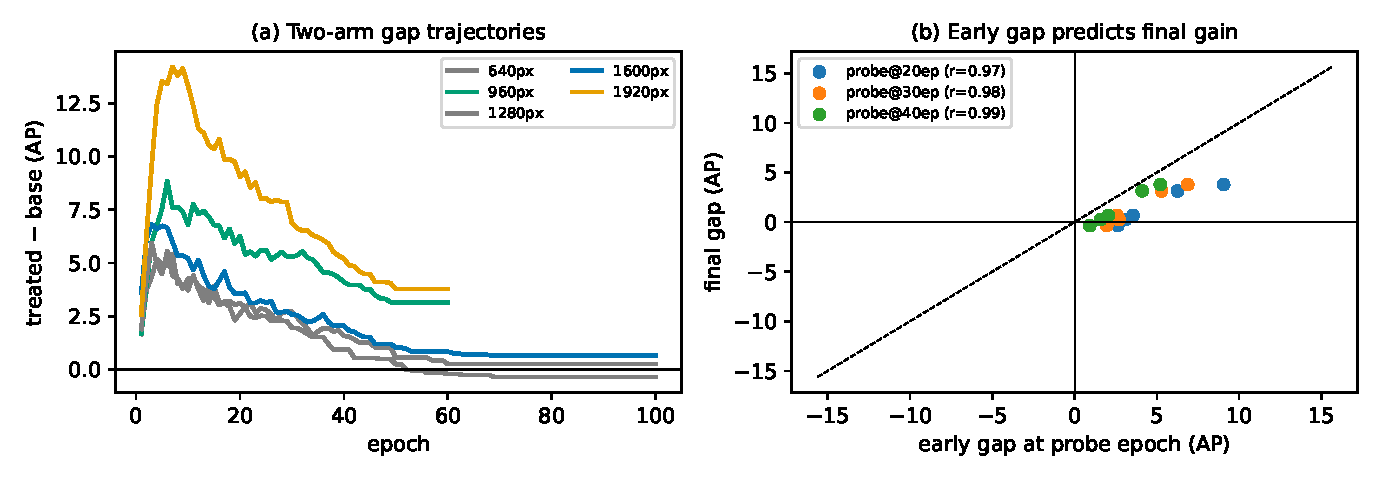
\includegraphics[width=\columnwidth]{figures/fig9_early_signal.pdf}
\caption{Retrospective early-signal analysis. (a) Best-checkpoint gap trajectories (rebalanced $-$ base) per resolution; (b) the 30-epoch probe gap versus eventual gain (descriptive $r{=}0.98$ over five completed cases; four pairs use union sampling, the 1280-px pair uses a legacy frequency proxy). The dashed $2.5$-\ap{} line is a post-hoc cut point that separates the observed larger-gap regimes from the volume-saturated 1280-px regime in $5/5$ completed cases; it is not a prospective-validation or universal-predictor claim.}
\label{fig:earlysignal}
\end{figure}

\begin{table}[!t]
\centering
\caption{Resolution--sampling ladder on the same YOLOv8m-P2 detector family (native protocol, md300, matched 60/100-epoch budgets per series). The 960-px cell is the new batch-matched re-evaluation; the 1280-px treated arm is a legacy frequency-sampling proxy, not the exact union policy. The effect tracks data-exposure headroom, not resolution alone. Exact same-evaluator md100 controls are reported separately in Table~\ref{tab:exactcontrols}, and native/md100 values are never subtracted.}
\label{tab:regimematrix}
\resizebox{\columnwidth}{!}{\begin{tabular}{lccccc}
\toprule
Resolution & 640 & 960 & 1280 & 1600 & 1920 \\
\midrule
Base \ap & 27.27 & 28.17$^{c}$ & 36.20 & 38.07 & 35.67 \\
Treated \ap & 27.48 & 31.98$^{c}$ & $\approx$36.25$^{d}$ & 38.85 & 39.50 \\
\midrule
$\Delta$ (same epoch) & $+0.21$ & $+3.81^{c}$ & $+0.05^{d}$ & $+0.78$ & $+3.83$ \\
$\Delta$ (exposure-matched) & --- & --- & --- & --- & $+0.49$ \\
Regime & unlearn. & under-fit & volume-sat. & sweet & expos.-lim. \\
\bottomrule
\multicolumn{6}{l}{\footnotesize $^{c}$new batch-matched 960 base/union re-evaluation (28.17/31.98 native; 28.10/31.92 md100).}\\
\multicolumn{6}{l}{\footnotesize $^{d}$legacy frequency-sampling proxy at 1280 ($36.25$ vs.\ $36.20$); exact triplet in Table~\ref{tab:exactcontrols}.}
\end{tabular}}
\end{table}

\begin{table}[!t]
\centering
\caption{Exact md100 rebalancing controls (same external evaluator; all values COCO md100). Volume $\Delta$ = random $-$ base; targeted $\Delta$ = union $-$ random. The 1600-px row reports mean$\pm$std over seeds ($n{=}3$ base, $n{=}5$ per sampling arm); the 1920-px row is the exposure-matched pair (base trained for 120 epochs vs.\ union for 60). Native and md100 protocols are never mixed in a subtraction.}
\label{tab:exactcontrols}
\resizebox{\columnwidth}{!}{\begin{tabular}{lccccc}
\toprule
Series & Base & Random & Union/Targeted & Vol.\ $\Delta$ & Tgt.\ $\Delta$ \\
\midrule
960 exact (batch 2, 60 ep) & 28.10 & 31.77 & 31.92 & $+3.67$ & $+0.15$ \\
1280 exact & 34.63 & 34.72 & 35.12 & $+0.09$ & $+0.40$ \\
1600 (seeds) & $36.55^{\pm.21}$ & $36.91^{\pm.29}$ & $37.18^{\pm.18}$ & $+0.36$ & $+0.28$ \\
1920 exposure-matched & $37.51^{\dagger}$ & --- & $37.93$ & --- & $+0.42$ \\
\bottomrule
\multicolumn{6}{l}{\footnotesize $^{\dagger}$base@120 epochs; union arm trained 60 epochs. Exposure-matched \aps{} residual $+0.92$.}
\end{tabular}}
\end{table}

\subsection{Cross-Dataset Transfer (\uavdt{})}
\label{sec:uavdt}
\begin{table}[!t]
\centering
\caption{Cross-dataset transfer on \uavdt{} (60 epochs; converged, best@23--29). Zero-shot profiler transfer: the same profiler is used without dataset-specific changes, while the final policy remains subject to the disclosed bounded search. Bold marks the best value in each metric.}
\label{tab:uavdt}
\begin{tabular}{lcc}
\toprule
Config & \ap & Tail (truck/bus) \\
\midrule
base & 37.86 & 32.05 \\
freq-only & 37.80 & 31.49 \\
union sampling & \textbf{38.55} & \textbf{33.73} \\
\bottomrule
\end{tabular}
\end{table}
Union sampling transfers ($+0.69$~\ap; tail $+1.69$) while frequency-only does not---consistent with the DAHP profile, since \uavdt{}'s confusion axis (car--van--truck, $\kappa{=}0.935$) dominates its long tail (Table~\ref{tab:uavdt}). This is a zero-shot \emph{profiler} transfer rather than a zero-shot policy-generalization claim: the transfer experiment still relies on the disclosed bounded search over the profiler-emitted candidates.

\subsection{Efficiency}
\label{sec:efficiency}

\begin{table*}[!t]
\centering
\caption{Stage-wise latency and memory on one exclusive desktop RTX~3090 (20 warm-up and 300 measured VisDrone-val images; batch 1, FP16, confidence $0.25$, CUDA synchronization after every image). End-to-end time is the aggregate wall time over 300 images; stage times come from Ultralytics \texttt{Results.speed}; ``pipeline'' is the end-to-end minus stage-sum accounting residual. Active/reserved CUDA memory is reported after warm-up. The host had 24 CPU cores and recorded 1-min load averages of 30.4 and 22.3 at benchmark start/end, so host-sensitive end-to-end timings are conservative. No value is bold because accuracy and latency prefer different configurations.}
\label{tab:efficiency}
\resizebox{\textwidth}{!}{\begin{tabular}{lccccccccc}
\toprule
Model & Input & End-to-end ms & FPS & Pre ms & Infer ms & Post ms & Pipeline ms & Params & VRAM act./res. \\
\midrule
Baseline v8m-P2 & 1280 & 26.1 & 38.3 & 5.8 & 12.3 & 1.5 & 6.5 & 25.0M & 0.17/0.31\,GB \\
$V_L$ (vanilla) & 1600 & 33.3 & 30.0 & 8.3 & 18.7 & 1.5 & 4.9 & 43.6M & 0.25/0.45\,GB \\
$V_L{+}P_2$ & 1600 & 39.6 & 25.3 & 8.6 & 24.4 & 1.6 & 5.1 & 42.8M & 0.35/0.67\,GB \\
\dahpL{} & 1600 & 38.0 & 26.3 & 7.3 & 24.4 & 1.5 & 4.8 & 42.8M & 0.35/0.67\,GB \\
\bottomrule
\end{tabular}}
\end{table*}

Table~\ref{tab:efficiency} reports the final 300-image protocol. \dahpL{} runs at $38.0$~ms image${^{-1}}$ ($26.3$~FPS) and has the same parameter count and active/reserved CUDA-memory footprint as $V_L{+}P_2$. The union-sampling policy inserts no inference-time module; the small latency difference between these same-architecture checkpoints is not claimed as a speedup and reflects measured input/pipeline variability. Because the CPU load exceeded the core count when the benchmark began, the end-to-end and preprocessing/pipeline columns are conservative; the inference-stage column is reported separately to reduce this ambiguity. These are desktop-GPU measurements, not edge-device deployment evidence. A literature claim of 110~FPS for \remdet{} on RTX~4090 uses different hardware and input settings and is therefore not subtracted or directly compared here.

\subsection{Qualitative Results}
Fig.~\ref{fig:radar} contrasts per-class \ap{} between the baseline and \dahpL{}; Fig.~\ref{fig:qual} shows hard-class-rich triplets (GT / baseline / ours): recovered \emph{awning-tricycle} and \emph{tricycle} detections and reduced \emph{car--van} confusion.

\begin{figure}[!t]
\centering
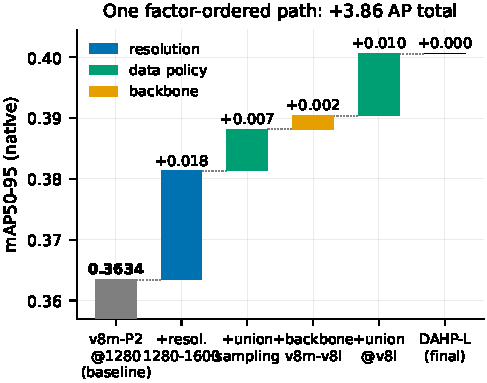
\includegraphics[width=\linewidth]{figures/fig2_waterfall.pdf}
\caption{One native-protocol path from the baseline to \dahpL{}. Increment labels are order-dependent path contributions; the controlled architecture/volume/targeting decomposition is given in Table~\ref{tab:attribution}.}
\label{fig:waterfall}
\end{figure}

\begin{figure*}[!t]
\centering
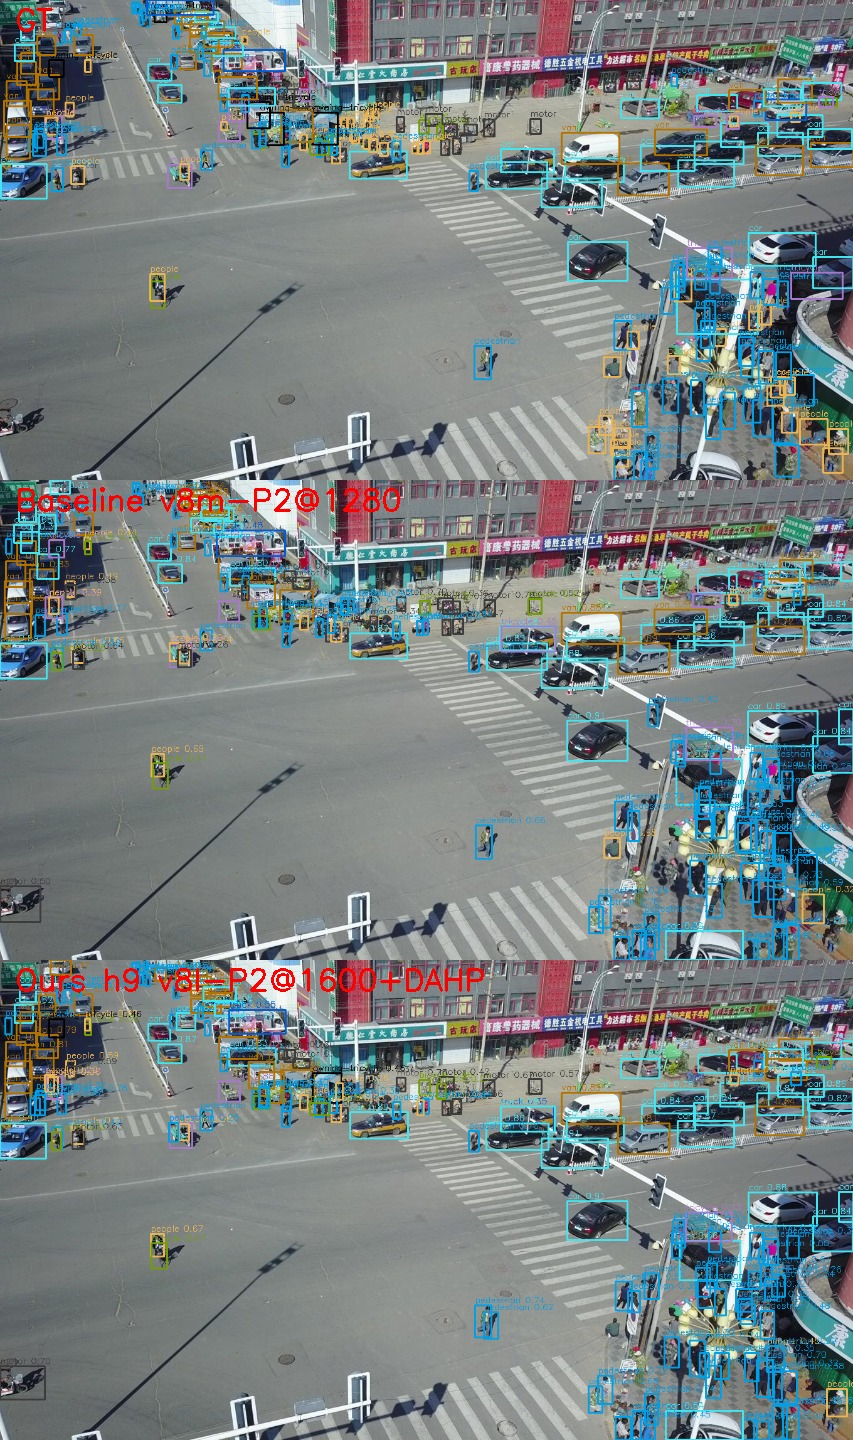
\includegraphics[width=0.49\textwidth]{qualitative/qual_0000291_01201_d_0000874.jpg}\hfill
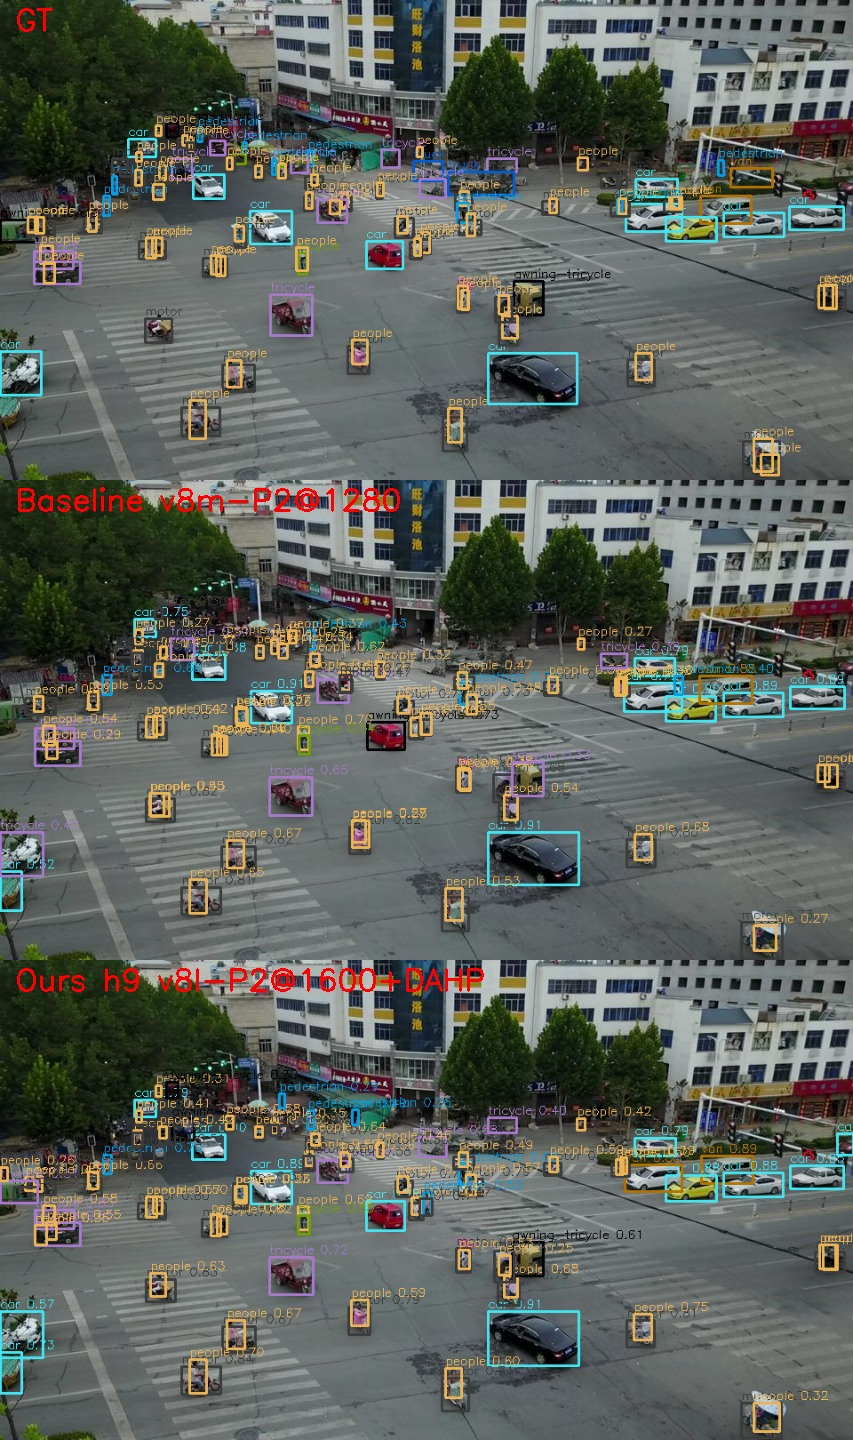
\includegraphics[width=0.49\textwidth]{qualitative/qual_0000193_01705_d_0000112.jpg}
\caption{Qualitative comparison on hard-class-rich validation images. Each triplet: ground truth (top), baseline v8m-P2@1280 (middle), \dahpL{} (bottom). \dahpL{} recovers missed awning-tricycle/tricycle instances and reduces car--van confusion.}
\label{fig:qual}
\end{figure*}

\begin{figure}[!t]
\centering
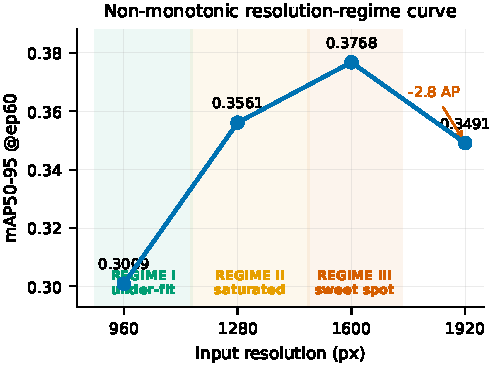
\includegraphics[width=\linewidth]{figures/fig4_resolution_regime.pdf}
\caption{Non-monotonic resolution-only ladder at matched epochs. The peak at $1600$\,px defines the sweet spot; the post-peak $1920$-px point and its exposure-limited sampling behavior are analyzed in Table~\ref{tab:regimematrix}.}
\label{fig:regime}
\end{figure}

\begin{figure}[!t]
\centering
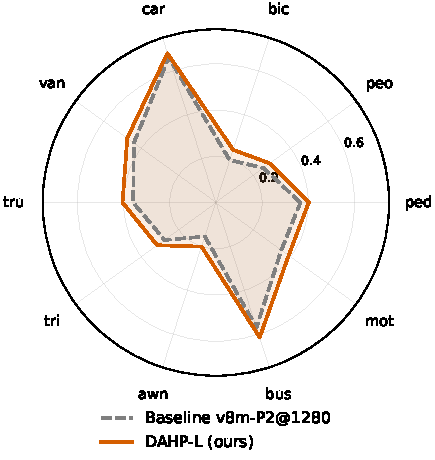
\includegraphics[width=\linewidth]{figures/fig5_radar.pdf}
\caption{Per-class \ap{}: baseline (grey, dashed) vs.\ ours (red, solid).}
\label{fig:radar}
\end{figure}


\begin{figure*}[!t]
\centering
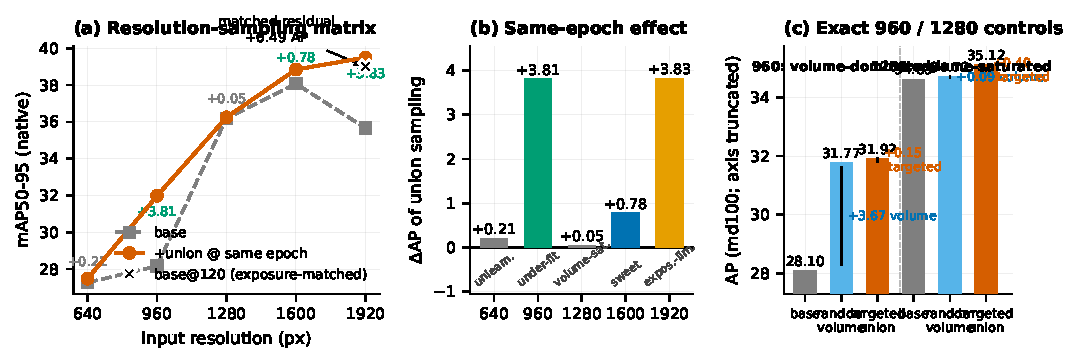
\includegraphics[width=\textwidth]{figures/fig8_regime_matrix.pdf}
\caption{The five-point resolution--sampling matrix. (a) Base vs.\ union sampling across resolutions under the legacy native protocol; (b) the same-epoch effect tracks data-exposure headroom, not resolution; (c) exact md100 triplets contrast the volume-dominated 960-px regime ($+3.67$ volume, $+0.15$ targeted) with the volume-saturated 1280-px regime ($+0.09$ volume, $+0.40$ targeted). The 1920 bar is an apparent same-epoch gain; the exposure-matched residual is $+0.49$ native / $+0.42$ md100 \ap.}
\label{fig:regimematrix}
\end{figure*}\begin{figure*}[!t]
\centering
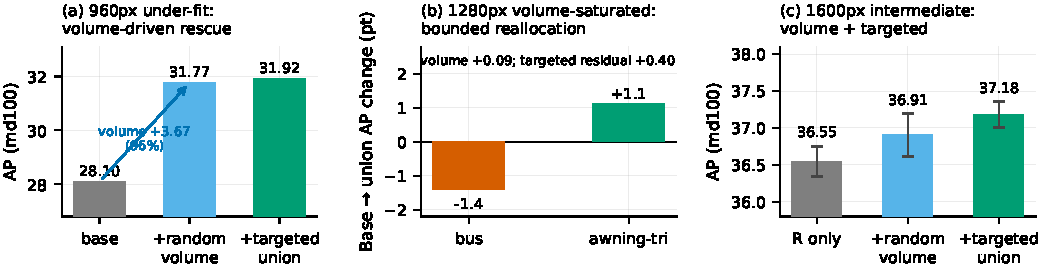
\includegraphics[width=\textwidth]{figures/fig7_regime_mechanism.pdf}
\caption{Mechanistic evidence for the regime principle: (a) volume-dominated tail rescue at 960\,px; (b) volume-saturated reallocation with a bounded targeted residual at 1280\,px; (c) positive-sum window at 1600\,px.}
\label{fig:mechanism}
\end{figure*}

\subsection{Negative Results}
\label{sec:negative}
All disclosed: full YOLO12-L/YOLO26-L@640 baselines (23.67/24.90~\ap); earlier YOLO26-family probes at 1280 ($25.6$--$33.5$~\ap); pure tiled inference on full-image models ($-2.3$ to $-2.6$); SAFT mixing ($37.76<$ pure TTA $37.96$); frequency sampling at $1280$ ($36.25\approx$ baseline); naive allocator ($38.51<$ union $38.85$); the full feature-module family---CSA/CCA/FBE single modules, their full combination, cls/box decoupling variants, and a P2 transfer ($-0.7$ to $+0.1$~\ap, val DFL $+0.05$--$0.08$; Table~\ref{tab:negative}).

\section{Discussion}
The regime principle implies that data-level rebalancing is not a universally positive intervention but an exposure-indexed tool: profile the label distribution first, then use bounded base/random probes and memory constraints to choose resolution/capacity before rebalancing. Three boundary conditions deserve emphasis. At 640\,px, tail objects are not learnable at the available stride, so duplication cannot rescue them---the principle has a lower bound set by learnability, not by sampling. At $1280$\,px, the volume channel is already saturated, but targeted union still retains a $+0.40$-\ap{} md100 residual over random duplication; saturation does not imply that every component of rebalancing is zero. At $1920$\,px, an apparently saturated run was in fact exposure-limited: doubling per-epoch exposure produced an apparent $+3.83$-\ap{} gain, but training the base for an exposure-matched 120 epochs recovered most of it, leaving a $+0.42$-\ap{} md100 residual concentrated on small objects. Practitioners should therefore diagnose \emph{why} a run has plateaued (capacity vs.\ exposure) before attributing a gain to rebalancing. In deployment terms, the practical recipe is: raise effective pixels until the exposure budget is the binding constraint, then rebalance. Limitations: (i) the principle is characterized on two UAV datasets and the YOLO family; the matched RT-DETR probe in Table~\ref{tab:crossfamily} reports a boundary rather than family independence; (ii) the compute-matched \remdet{} retrain bounds what any single 24-GB GPU achieves with that architecture at $1600$\,px but does not measure its 8-GPU recipe; (iii) the WBF ensemble trades parameters for accuracy and is reported separately from the single-model claim; and (iv) VisDrone conclusions are limited to the validation split because official test-dev ground truth was unavailable.

\section{Conclusion}
A label-only profiler, a regime-indexed rebalancing principle, and a policy-level non-invasive recipe deliver the strongest reproduced result among the evaluated VisDrone-val configurations ($40.06$~\ap{} native / $38.16$~\ap{} COCO protocol; $39.61$~\ap{} fused), transferable gains on \uavdt{}, and a documented failure map of both the architectural alternative and an out-of-family transfer attempt. The evidence supports an exposure-aware principle for the studied YOLO policies, not a universal rebalancing rule or an official test-dev benchmark claim. The single model uses 42.8M parameters (58\% of \remdet{}); the sampling policy itself leaves detector inference unchanged.

\section*{Data and Code Availability}
\visdrone{} and \uavdt{} are publicly released by their respective challenge organizers. This study uses the VisDrone validation split; no official test-dev ground truth is used. The profiler, rebalanced-dataset builders, threshold-sensitivity audit, evaluation and latency scripts, LaTeX source, figures, configs, and a sanitized metric-summary JSON are available at \url{https://github.com/AirAI-Lab/DAHP-UAV-Detection}. Prediction dumps and machine-specific paths are omitted from the public artifact; every released table value is traceable to the sanitized result file or documented log provenance.

\appendix
\begin{table*}[!t]
\centering
\caption{Per-class AP for key configurations (native protocol). UAVDT rows use its 4-class vehicle taxonomy.}
\label{tab:perclass}
\resizebox{\textwidth}{!}{%
\begin{tabular}{lcccccccccc}
\toprule
Configuration & ped & peo & bic & car & van & tru & tri & awn & bus & mot \\
\midrule
Baseline v8m-P2@1280 & 36.6 & 25.4 & 19.3 & 66.0 & 43.9 & 35.8 & 27.6 & 15.5 & 56.9 & 35.0 \\
R only (v8m-P2@1600) & 38.7 & 27.3 & 21.9 & 67.0 & 45.5 & 37.3 & 29.1 & 18.8 & 58.2 & 37.0 \\
DAHP-M (R+T$\cup$C) & 39.0 & 27.5 & 22.0 & 67.4 & 46.8 & 38.8 & 31.1 & 18.7 & 59.4 & 37.9 \\
$V_L$ (v8l no-P2@1600) & 37.6 & 26.1 & 22.0 & 66.7 & 44.5 & 39.2 & 30.1 & 18.0 & 58.4 & 36.9 \\
$V_L{+}P_2$ & 39.0 & 27.5 & 23.4 & 67.6 & 46.6 & 38.9 & 31.4 & 18.8 & 59.7 & 37.5 \\
\textbf{DAHP-L} & 40.2 & 28.8 & 24.0 & 67.9 & 47.4 & 40.4 & 31.4 & 20.1 & 61.4 & 38.9 \\
DAHP-L seed43 & 40.4 & 29.0 & 24.1 & 67.9 & 47.0 & 39.9 & 31.3 & 19.6 & 58.9 & 38.9 \\
UAVDT base & --- & --- & --- & 50.7 & 36.7 & 14.9 & --- & --- & 49.2 & --- \\
% missing perclass_uavdt_cf.json
\bottomrule
\end{tabular}}
\end{table*}

\begin{thebibliography}{42}
\bibitem{visdrone} P. Zhu, L. Wen, D. Du, X. Bian, H. Fan, Q. Hu, and H. Ling, ``Detection and tracking meet drones challenge,'' \emph{IEEE Trans. Pattern Anal. Mach. Intell.}, vol. 44, no. 11, pp. 7380--7399, 2022, doi: 10.1109/TPAMI.2021.3119563.
\bibitem{uavdt} D. Du, Y. Qi, H. Yu, Y. Yang, K. Duan, G. Li, W. Zhang, Q. Huang, and Q. Tian, ``The unmanned aerial vehicle benchmark: Object detection and tracking,'' in \emph{Proc. Eur. Conf. Comput. Vis.}, pp. 375--391, 2018, doi: 10.1007/978-3-030-01249-6\_23.
\bibitem{clusdet} F. Yang, H. Fan, P. Chu, E. Blasch, and H. Ling, ``Clustered object detection in aerial images,'' in \emph{Proc. IEEE/CVF Conf. Comput. Vis. Pattern Recognit.}, pp. 8310--8319, 2019, doi: 10.1109/ICCV.2019.00840.
\bibitem{dmnet} C. Li, T. Yang, S. Zhu, C. Chen, and S. Guan, ``Density map guided object detection in aerial images,'' in \emph{Proc. IEEE/CVF Conf. Comput. Vis. Pattern Recognit. Workshops}, pp. 737--746, 2020, doi: 10.1109/CVPRW50498.2020.00103.
\bibitem{ufpmp} Y. Huang, J. Chen, and D. Huang, ``UFPMP-Det: Toward accurate and efficient object detection on drone imagery,'' \emph{Proc. AAAI Conf. Artif. Intell.}, vol. 36, no. 1, pp. 1026--1033, 2022, doi: 10.1609/aaai.v36i1.19986.
\bibitem{czdet} A. Meethal, E. Granger, and M. Pedersoli, ``Cascaded zoom-in detector for high resolution aerial images,'' in \emph{Proc. IEEE/CVF Conf. Comput. Vis. Pattern Recognit. Workshops}, pp. 2046--2055, 2023, doi: 10.1109/CVPRW59228.2023.00198.
\bibitem{amrnet} Z. Wei, C. Duan, X. Song, Y. Tian, and H. Wang, ``AMRNet: Chips augmentation in aerial images object detection,'' arXiv:2009.07168, 2020, doi: 10.48550/arXiv.2009.07168.
\bibitem{tph} X. Zhu, S. Lyu, X. Wang, and Q. Zhao, ``TPH-YOLOv5: Improved YOLOv5 based on transformer prediction head for object detection on drone-captured scenarios,'' in \emph{Proc. IEEE/CVF Int. Conf. Comput. Vis. Workshops}, pp. 2778--2788, 2021, doi: 10.1109/ICCVW54120.2021.00312.
\bibitem{sahi} F. C. Akyon, S. O. Altinuc, and A. Temizel, ``Slicing aided hyper inference and fine-tuning for small object detection,'' in \emph{Proc. IEEE Int. Conf. Image Process.}, pp. 966--970, 2022, doi: 10.1109/ICIP46576.2022.9897990.
\bibitem{remdet} C. Li, R. Zhao, Z. Wang, H. Xu, and X. Zhu, ``RemDet: Rethinking efficient model design for UAV object detection,'' \emph{Proc. AAAI Conf. Artif. Intell.}, vol. 39, no. 5, pp. 4643--4651, 2025, doi: 10.1609/aaai.v39i5.32490.
\bibitem{uavdetr} H. Zhang, K. Liu, Z. Gan, and G.-N. Zhu, ``UAV-DETR: Efficient end-to-end object detection for unmanned aerial vehicle imagery,'' arXiv:2501.01855, 2025, doi: 10.48550/arXiv.2501.01855.
\bibitem{aqfnet} Y. He, Y. Tang, R. Xiao, and Y. Pang, ``AQF-Net: Adaptive query modeling and efficient feature fusion for UAV tiny-object detection,'' \emph{PLoS One}, vol. 21, no. 8, art. no. e0355299, 2026, doi: 10.1371/journal.pone.0355299.
\bibitem{uavdetmamba} Y. Yang, F. Guo, and P. Niu, ``UAVDet: A CNN--Mamba hybrid network for efficient small object detection in UAV imagery,'' \emph{Comput. Vis. Image Underst.}, vol. 264, art. no. 104637, 2026, doi: 10.1016/j.cviu.2026.104637.
\bibitem{casanet} K. Zheng, Y. Zhong, W. Song, and Q. Jiang, ``CASA-Net: Context-aware small-object adaptation network for UAV aerial images,'' \emph{Remote Sens.}, vol. 18, no. 14, art. no. 2327, 2026, doi: 10.3390/rs18142327.
\bibitem{doldetr} S. Chen and Z. Li, ``DOL-DETR: An efficient small object detection algorithm for unmanned aerial vehicle remote sensing,'' \emph{Appl. Sci.}, vol. 16, no. 9, art. no. 4510, 2026, doi: 10.3390/app16094510.
\bibitem{lgidetr} Z. Chen, ``LGI-DETR: Local-global interaction for UAV object detection,'' arXiv:2503.18785, 2025, doi: 10.48550/arXiv.2503.18785.
\bibitem{querydet} C. Yang, Z. Huang, and N. Wang, ``QueryDet: Cascaded sparse query for accelerating high-resolution small object detection,'' in \emph{Proc. IEEE/CVF Conf. Comput. Vis. Pattern Recognit.}, pp. 13658--13667, 2022, doi: 10.1109/CVPR52688.2022.01330.
\bibitem{ceasc} B. Du, Y. Huang, J. Chen, and D. Huang, ``Adaptive sparse convolutional networks with global context enhancement for faster object detection on drone images,'' in \emph{Proc. IEEE/CVF Conf. Comput. Vis. Pattern Recognit.}, pp. 13435--13444, 2023, doi: 10.1109/CVPR52729.2023.01291.
\bibitem{goldyolo} C. Wang, W. He, Y. Nie, J. Guo, C. Liu, Y. Wang, and K. Han, ``Gold-YOLO: Efficient object detector via gather-and-distribute mechanism,'' in \emph{Adv. Neural Inf. Process. Syst.}, vol. 36, pp. 51094--51112, 2023, doi: 10.52202/075280-2224.
\bibitem{rtdetr} Y. Zhao, W. Lv, S. Xu, J. Wei, G. Wang, Q. Dang, Y. Liu, and J. Chen, ``DETRs beat YOLOs on real-time object detection,'' in \emph{Proc. IEEE/CVF Conf. Comput. Vis. Pattern Recognit.}, pp. 16965--16974, 2024, doi: 10.1109/CVPR52733.2024.01605.
\bibitem{rtdetrv2} Y. Zhao, W. Lv, S. Xu, J. Wei, G. Wang, Q. Dang, Y. Liu, and J. Chen, ``RT-DETRv2: Improved baseline with bag-of-freebies for real-time detection transformer,'' arXiv:2407.17140, 2024, doi: 10.48550/arXiv.2407.17140.
\bibitem{dfine} Y. Peng, H. Li, P. Wu, Y. Zhang, X. Sun, and F. Wu, ``D-FINE: Redefine regression task in DETRs as fine-grained distribution refinement,'' arXiv:2410.13842, 2024, doi: 10.48550/arXiv.2410.13842.
\bibitem{yolov8} G. Jocher and A. Chaurasia, ``Ultralytics YOLOv8,'' Ultralytics, 2023. [Online]. Available: \url{https://docs.ultralytics.com/models/yolov8/}. Accessed: Sep. 15, 2026.
\bibitem{frcnn} S. Ren, K. He, R. Girshick, and J. Sun, ``Faster R-CNN: Towards real-time object detection with region proposal networks,'' \emph{IEEE Trans. Pattern Anal. Mach. Intell.}, vol. 39, no. 6, pp. 1137--1149, 2017, doi: 10.1109/TPAMI.2016.2577031.
\bibitem{cbloss} Y. Cui, M. Jia, T.-Y. Lin, Y. Song, and S. Belongie, ``Class-balanced loss based on effective number of samples,'' in \emph{Proc. IEEE/CVF Conf. Comput. Vis. Pattern Recognit.}, pp. 9260--9269, 2019, doi: 10.1109/CVPR.2019.00949.
\bibitem{eqlv2} J. Tan, X. Lu, G. Zhang, C. Yin, and Q. Li, ``Equalization loss v2: A new gradient balance approach for long-tailed object detection,'' in \emph{Proc. IEEE/CVF Conf. Comput. Vis. Pattern Recognit.}, pp. 1685--1694, 2021, doi: 10.1109/CVPR46437.2021.00173.
\bibitem{seesaw} J. Wang, W. Zhang, Y. Zang, Y. Cao, J. Pang, T. Gong, K. Chen, Z. Liu, C. C. Loy, and D. Lin, ``Seesaw loss for long-tailed instance segmentation,'' in \emph{Proc. IEEE/CVF Conf. Comput. Vis. Pattern Recognit.}, pp. 9690--9699, 2021, doi: 10.1109/CVPR46437.2021.00957.
\bibitem{bge} Y. Li, T. Wang, B. Kang, S. Tang, C. Wang, J. Li, and J. Feng, ``Overcoming classifier imbalance for long-tail object detection with balanced group softmax,'' in \emph{Proc. IEEE/CVF Conf. Comput. Vis. Pattern Recognit.}, pp. 10988--10997, 2020, doi: 10.1109/CVPR42600.2020.01100.
\bibitem{dbloss} T. Wu, Q. Huang, Z. Liu, Y. Wang, and D. Lin, ``Distribution-balanced loss for multi-label classification in long-tailed datasets,'' in \emph{Proc. Eur. Conf. Comput. Vis.}, pp. 162--178, 2020, doi: 10.1007/978-3-030-58548-8\_10.
\bibitem{rfs} A. Gupta, P. Dollár, and R. Girshick, ``LVIS: A dataset for large vocabulary instance segmentation,'' in \emph{Proc. IEEE/CVF Conf. Comput. Vis. Pattern Recognit.}, pp. 5351--5359, 2019, doi: 10.1109/CVPR.2019.00550.
\bibitem{addet} Z. Li, S. Lian, D. Pan, Y. Wang, and W. Liu, ``AD-Det: Boosting object detection in UAV images with focused small objects and balanced tail classes,'' \emph{Remote Sens.}, vol. 17, no. 9, art. no. 1556, 2025, doi: 10.3390/rs17091556.
\bibitem{eirfs} T. Ahmed, A. Kumar, C. Álvarez Casado, A. Zhang, T. Hänninen, L. Loven, M. B. López, and S. Tarkoma, ``Exponentially weighted instance-aware repeat factor sampling for long-tailed object detection model training in unmanned aerial vehicle surveillance scenarios,'' arXiv:2503.21893, 2025, doi: 10.48550/arXiv.2503.21893.
\bibitem{ldam} Z. Liu, Z. Miao, X. Zhan, J. Wang, B. Gong, and S. X. Yu, ``Learning imbalanced datasets with label-distribution-aware margin loss,'' in \emph{Adv. Neural Inf. Process. Syst.}, vol. 32, 2019.
\bibitem{wbf} R. Solovyev, W. Wang, and T. Gabruseva, ``Weighted boxes fusion: Ensembling boxes from different object detection models,'' \emph{Image Vis. Comput.}, vol. 107, art. no. 104117, 2021, doi: 10.1016/j.imavis.2021.104117.
\bibitem{coco} T.-Y. Lin, M. Maire, S. Belongie, J. Hays, P. Perona, D. Ramanan, P. Dollár, and C. L. Zitnick, ``Microsoft COCO: Common objects in context,'' in \emph{Proc. Eur. Conf. Comput. Vis.}, pp. 740--755, 2014, doi: 10.1007/978-3-319-10602-1\_48.
\bibitem{focal} T.-Y. Lin, P. Goyal, R. Girshick, K. He, and P. Dollár, ``Focal loss for dense object detection,'' in \emph{Proc. IEEE Int. Conf. Comput. Vis.}, pp. 2999--3007, 2017, doi: 10.1109/ICCV.2017.324.
\bibitem{fcos} Z. Tian, C. Shen, H. Chen, and T. He, ``FCOS: Fully convolutional one-stage object detection,'' in \emph{Proc. IEEE/CVF Int. Conf. Comput. Vis.}, pp. 9626--9635, 2019, doi: 10.1109/ICCV.2019.00972.
\bibitem{gfl} X. Li, W. Wu, L. Wu, S. Chen, X. Hu, J. Li, J. Tang, and J. Yang, ``Generalized focal loss: Learning qualified and distributed bounding boxes for dense object detection,'' in \emph{Adv. Neural Inf. Process. Syst.}, vol. 33, 2020.
\bibitem{deform} J. Dai, H. Qi, Y. Xiong, Y. Li, G. Zhang, H. Hu, and Y. Wei, ``Deformable convolutional networks,'' in \emph{Proc. IEEE Int. Conf. Comput. Vis.}, pp. 764--773, 2017, doi: 10.1109/ICCV.2017.89.
\bibitem{yolo11} G. Jocher and Q. Jin, ``Ultralytics YOLO11,'' Ultralytics, 2024. [Online]. Available: \url{https://docs.ultralytics.com/models/yolo11/}. Accessed: Sep. 15, 2026.
\bibitem{yolo12} Y. Tian, Q. Ye, and D. Doermann, ``YOLOv12: Attention-centric real-time object detectors,'' arXiv:2502.12524, 2025, doi: 10.48550/arXiv.2502.12524.
\bibitem{yolo26} G. Jocher, J. Qiu, M. Liu, S. Lyu, F. C. Akyon, and M. E. Kalfaoglu, ``Ultralytics YOLO26: Unified real-time end-to-end vision models,'' arXiv:2606.03748, 2026, doi: 10.48550/arXiv.2606.03748.
\end{thebibliography}

\end{document}
